\documentclass[12pt]{article}

\usepackage[margin=2.5cm]{geometry}
\usepackage{graphicx}
\usepackage{lscape}

\usepackage{amsmath}

\renewcommand{\bottomfraction}{.9}
\renewcommand{\topfraction}{.9}
\renewcommand{\textfraction}{0.1}
\renewcommand{\floatpagefraction}{.9}


\begin{document}

\begin{center}
\large\textbf{Supporting Information for ``Maximum allowed solvent accessibilites of residues in proteins''}\\
\end{center}

\bigskip
\noindent Matthew Z. Tien, Austin G. Meyer, Dariya K. Sydykova, Stephanie J. Spielman, Claus O. Wilke

\bigskip

\subsection*{Supporting Figures}
\centerline{\includegraphics[width=6in]{figures/Ala_Rama_HSV_ALL_edited.pdf}}

\noindent Figure S1. Ramachandran plots for empirical and theoretical maximum SA values of alanine. (A) Empirical maximum SA values for each $5^\circ$ by $5^\circ$ bin. All non-empty bins are shown. (B) Theoretical maximum SA values, as determined by computational modeling, shown for non-empty bins in (A).

\vspace*{.5in}

\centerline{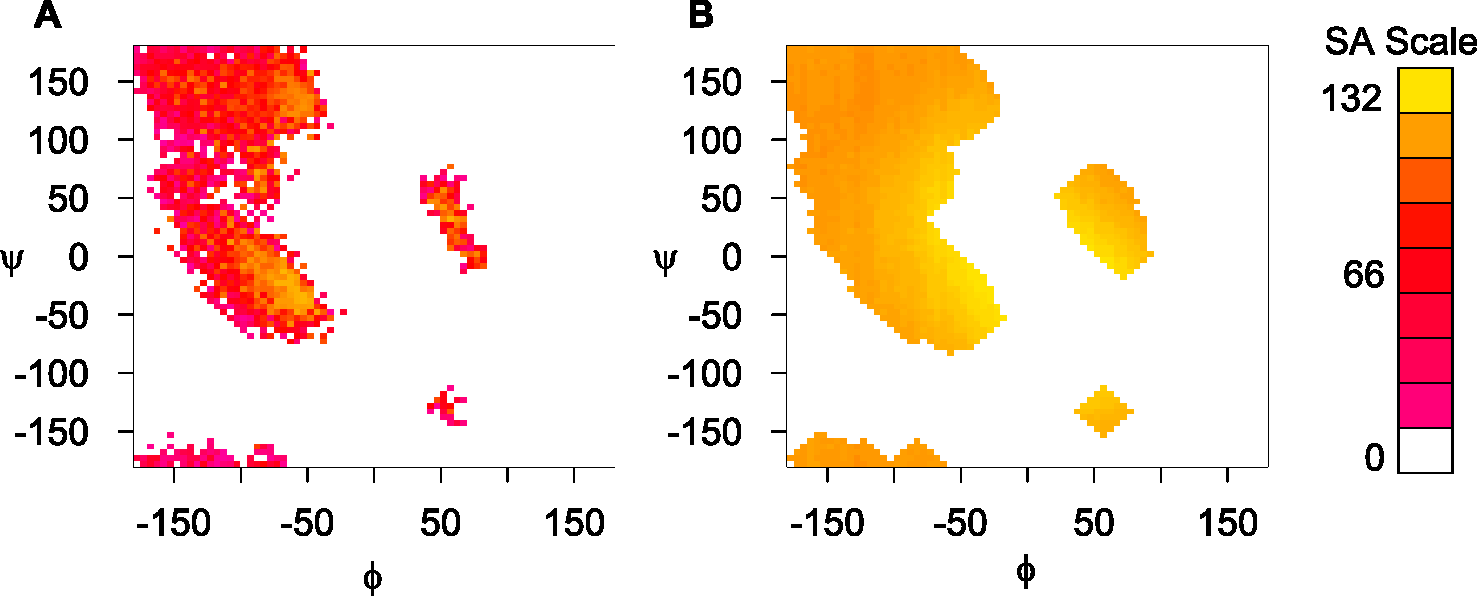
\includegraphics[width=6in]{figures/Ala_Rama_HSV_GENEROUS_edited.pdf}}

\noindent Figure S2. Ramachandran plots for empirical and theoretical maximum SA values of alanine. (A) Empirical maximum SA values for each $5^\circ$ by $5^\circ$ bin. All non-empty bins in the GENEROUS regions are shown. (B) Theoretical maximum SA values, as determined by computational modeling, shown for all bins in the GENEROUS region.

\newpage

\centerline{\includegraphics[width=6in]{figures/Ala_Rama_HSV_CORE_edited.pdf}}

\noindent Figure S3. Ramachandran plots for empirical and theoretical maximum SA values of alanine. (A) Empirical maximum SA values for each $5^\circ$ by $5^\circ$ bin. All bins in the CORE region are shown. (B) Theoretical maximum SA values, as determined by computational modeling, shown for all bins in the CORE region.


\vspace*{.5in}

\centerline{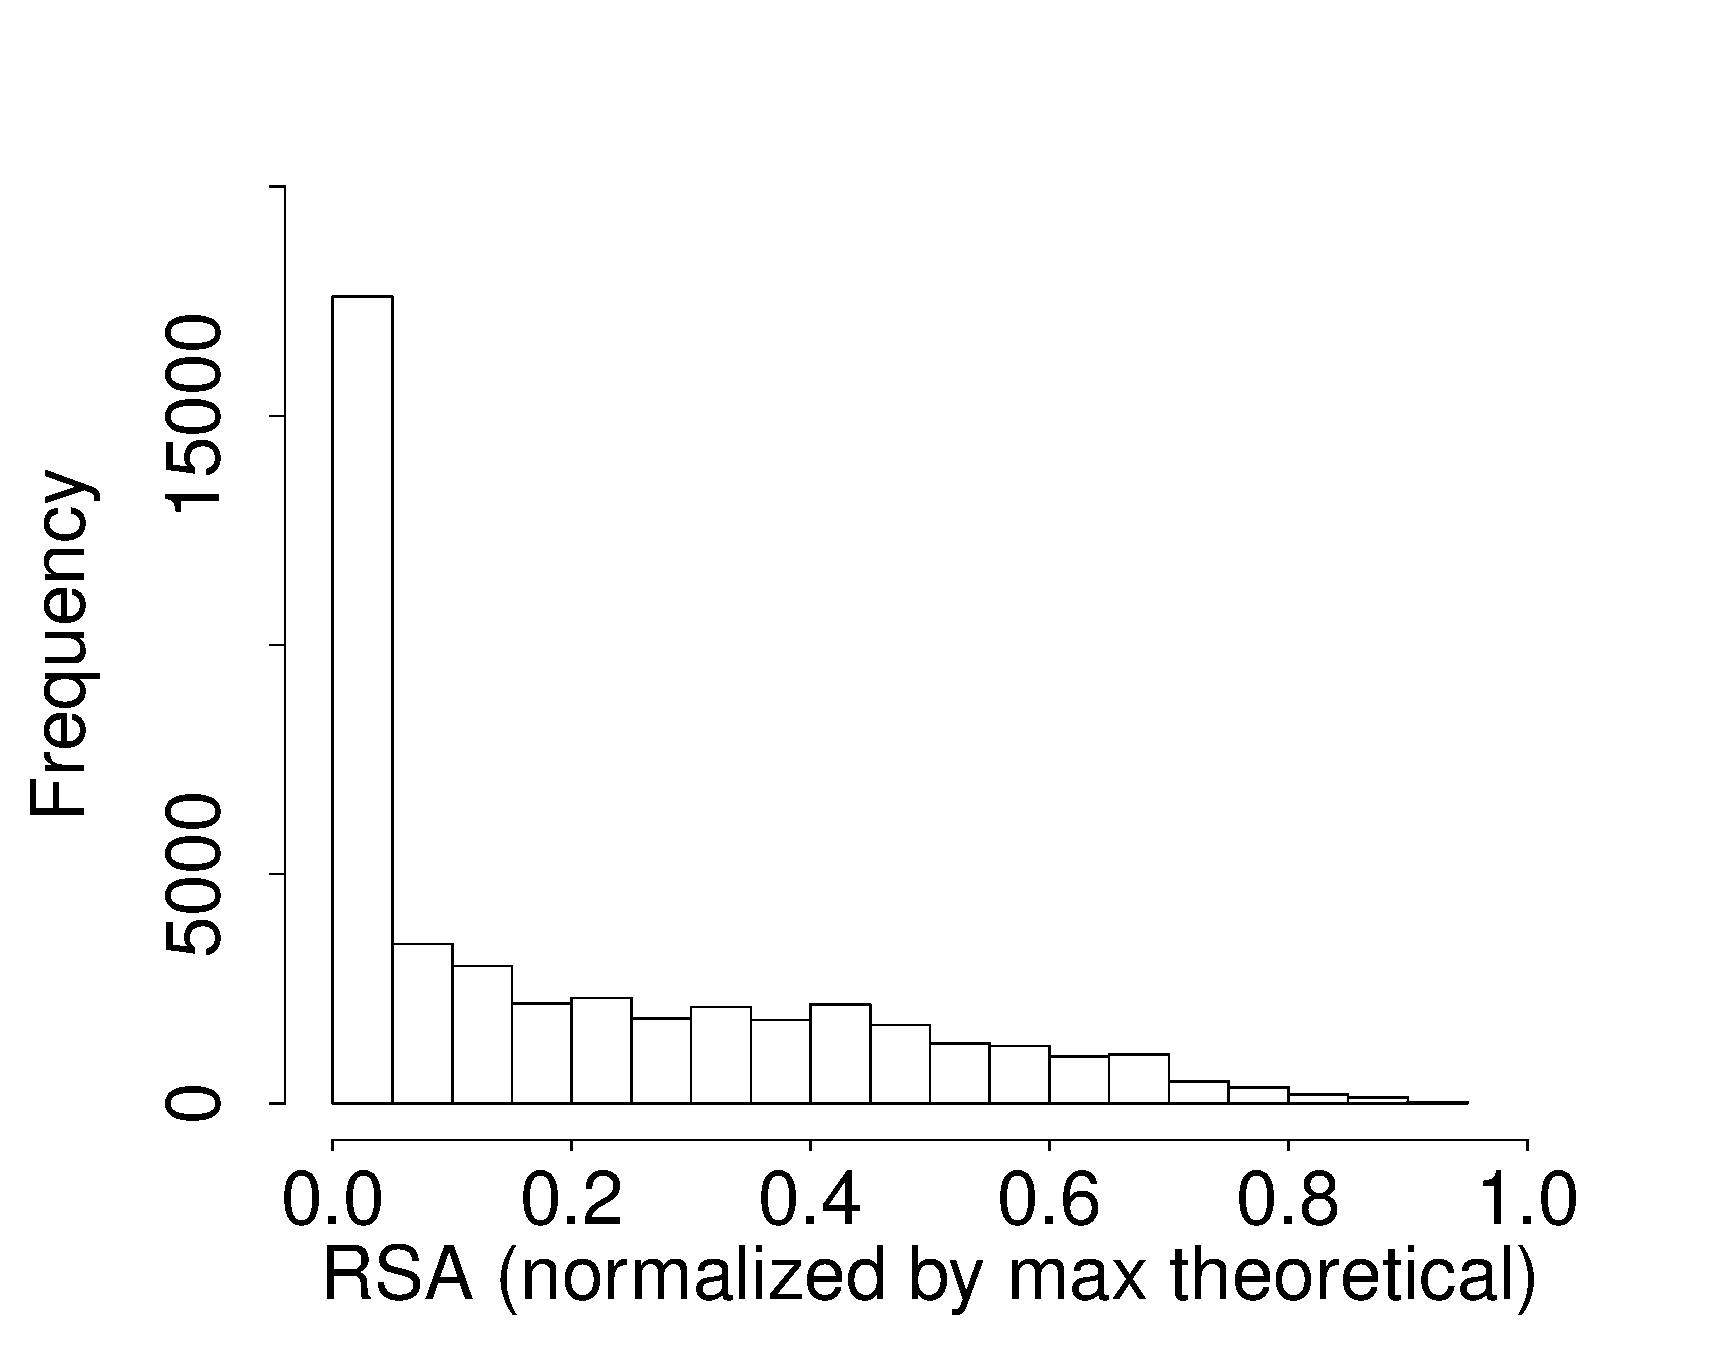
\includegraphics[width=3.5in]{figures/Alanine_RSA_distribution.pdf}}

\noindent Figure S4. Distribution of RSA values for alanine. RSA was calculated using our theoretically determined normalization values. This distribution is highly non-normal with a strong right skew. Therefore, mean RSA is a poor measure of center for this distribution. Similarly skewed distributions are found for most amino acids.

\newpage


\subsection*{Supporting Tables}



\noindent Table S1. Maximum SA values (in \AA$^2$) observed in the empirical and the theoretical data sets.

\begin{center}
\scriptsize
\begin{tabular}{lccccccccc}
 & \multicolumn{4}{c}{Empirical} &&\multicolumn{4}{c}{Theoretical}\\\cline{2-5}\cline{7-10}\\[-1.6ex]
Residue          & ALL & GENEROUS & ALLOWED & CORE & & ALL & GENEROUS & ALLOWED & CORE\\
\hline Alanine   & $121$ & $121$ & $121$ & $121$ & & $138$ & $132$ & $129$ & $128$\\
Arginine         & $265$ & $265$ & $265$ & $265$ & & $285$ & $280$ & $274$ & $274$\\
Asparagine       & $187$ & $187$ & $187$ & $187$ & & $204$ & $199$ & $195$ & $193$\\
Aspartate        & $187$ & $187$ & $187$ & $187$ & & $204$ & $197$ & $193$ & $192$\\
Cysteine         & $148$ & $148$ & $148$ & $133$ & & $169$ & $167$ & $167$ & $157$\\
Glutamate        & $214$ & $214$ & $214$ & $214$ & & $233$ & $227$ & $223$ & $222$\\
Glutamine        & $214$ & $214$ & $214$ & $214$ & & $234$ & $228$ & $225$ & $224$\\
Glycine          & $\phantom{0}97$ & $\phantom{0}97$ & $\phantom{0}97$ & $\phantom{0}97$ & & $114$ & $109$ & $104$ & $104$\\
Histidine        & $216$ & $216$ & $216$ & $216$ & & $231$ & $228$ & $224$ & $219$\\
Isoleucine       & $195$ & $195$ & $195$ & $195$ & & $208$ & $201$ & $197$ & $196$\\
Leucine          & $191$ & $191$ & $191$ & $191$ & & $211$ & $205$ & $201$ & $199$\\
Lysine           & $230$ & $230$ & $230$ & $229$ & & $246$ & $240$ & $236$ & $235$\\
Methionine       & $203$ & $203$ & $203$ & $203$ & & $227$ & $226$ & $224$ & $218$\\
Phenylalanine    & $228$ & $228$ & $228$ & $226$ & & $251$ & $244$ & $240$ & $236$\\
Proline          & $154$ & $154$ & $154$ & $154$ & & $166$ & $164$ & $159$ & $157$\\
Serine           & $143$ & $143$ & $143$ & $143$ & & $161$ & $158$ & $155$ & $150$\\
Threonine        & $163$ & $163$ & $163$ & $161$ & & $182$ & $176$ & $172$ & $171$\\
Tryptophan       & $264$ & $264$ & $264$ & $262$ & & $295$ & $293$ & $285$ & $282$\\
Tyrosine         & $255$ & $255$ & $255$ & $255$ & & $274$ & $266$ & $263$ & $262$\\
Valine           & $166$ & $166$ & $165$ & $165$ & & $184$ & $177$ & $174$ & $173$\\
\hline
\end{tabular}
\end{center}


\newpage
\noindent Table S2. Backbone conformation of maximally exposed trimer structures. Multiple rows per residue indicate alternative conformations with comparable solvent exposure.


\begin{center}
\footnotesize
\begin{tabular}{lccccc}
&  \multicolumn{2}{c}{Empirical} & ~~~& \multicolumn{2}{c}{Theoretical}\\\cline{2-3}\cline{5-6}
Residue & $\phi$ & $\psi$ & & $\phi$ & $\psi$ \\
\hline Alanine   & $-66.7^{\circ}$ & $-13.1^{\circ}$ & & $-60^{\circ}$ & $-15^{\circ}$\\
                 & $-52.1^{\circ}$ & $-33.6^{\circ}$ & &\\
                 & $-51.9^{\circ}$ & $-37.9^{\circ}$ & &\\
Arginine         & $-79.2^{\circ}$ & $-20.2^{\circ}$ & & $-70^{\circ}$ & ~\,$-5^{\circ}$ \\
		 &	&	& & $-70^{\circ}$ & $-25^{\circ}$\\
		 &	&	& & $-60^{\circ}$ & $-15^{\circ}$ to $-10^{\circ}$\\
		 &	&	& & $-55^{\circ}$ & $-30^{\circ}$\\
                 &      &       & & $-40^{\circ}$ & $-50^{\circ}$\\      
Asparagine       & $-94.8^{\circ}$ & ~\,$-3.4^{\circ}$ & & $-50^{\circ}$ & $-40^{\circ}$ \\
                 &      &       & & $-50^{\circ}$ & $-30^{\circ}$\\
		 &      &       & & $\phantom{-}70^{\circ}$ & ~\,$-5^{\circ}$\\
Aspartate        & $-79.4^{\circ}$ & $\phantom{-}83.0^{\circ}$ & & $\phantom{-}70^{\circ}$ & ~\,$-5^{\circ}$ \\
Cysteine         & $-87.7^{\circ}$ & $-45.1^{\circ}$ & & $\phantom{-}60^{\circ}$ & $-40^{\circ}$ \\
Glutamate        & $-55.0^{\circ}$ & $-49.9^{\circ}$ & & $-60^{\circ}$ & $-15^{\circ}$\\
Glutamine        & $-65.5^{\circ}$ & $-24.0^{\circ}$ & & $\phantom{-}70^{\circ}$ & ~\,$-5^{\circ}$\\
Glycine          & $\phantom{-}80.2^{\circ}$ & ~\,$\phantom{-}7.2^{\circ}$ & & $-75^{\circ}$ & $\phantom{-}20^{\circ}$  \\
                 &      &       & & $-75^{\circ}$ & $\phantom{-}50^{\circ}$\\
                 &      &       & & $-70^{\circ}$ & ~\,$\phantom{-}0^{\circ}$\\
                 &      &       & & $-65^{\circ}$ & $-10^{\circ}$\\
                 &      &       & & $-60^{\circ}$ & $-15^{\circ}$\\
                 &      &       & & $-50^{\circ}$ & $-25^{\circ}$\\
                 &      &       & & $\phantom{-}70^{\circ}$ & $-15^{\circ}$\\
                 &      &       & & $\phantom{-}75^{\circ}$ & $-30^{\circ}$\\
Histidine        & $\phantom{-}51.2^{\circ}$ & $\phantom{-}32.4^{\circ}$ & & $\phantom{-}65^{\circ}$ & $-25^{\circ}$  \\
		 &	 &	& & $\phantom{-}70^{\circ}$ & $-50^{\circ}$ \\
Isoleucine      & $-64.1^{\circ}$ & $-21.9^{\circ}$ & & $-55^{\circ}$ & $-25^{\circ}$ \\
		&	&	& & $-50^{\circ}$ & $-40^{\circ}$ \\
Leucine         & $-81.6^{\circ}$ & $-13.5^{\circ}$ & & $-70^{\circ}$ &  ~\,$-5^{\circ}$  \\
                & $-63.5^{\circ}$ & $-44.5^{\circ}$ & & & \\
                & $-60.9^{\circ}$ & $-29.3^{\circ}$ & & & \\
                & $-55.8^{\circ}$ & $-36.4^{\circ}$ & & & \\     
Lysine          & $\phantom{-}63.1^{\circ}$ & $\phantom{-}23.1^{\circ}$ & & $-45^{\circ}$ & $-45^{\circ}$ to $-40^{\circ}$ \\
Methionine      & $-67.5^{\circ}$ & $-27.5^{\circ}$ & & $\phantom{-}50^{\circ}$ & $-40^{\circ}$  \\
Phenylalanine   & $-50.3^{\circ}$ & \,\,$135.2^{\circ}$ & & $-45^{\circ}$ & $-40^{\circ}$  \\
                &       &       & & $\phantom{-}70^{\circ}$ & $-10^{\circ}$ \\
Proline         &  $-63.8^{\circ}$ & $-21.6^{\circ}$ & & $-55^{\circ}$ & $-20^{\circ}$  \\
Serine          & $-58.1^{\circ}$ & $-27.3^{\circ}$ & & $\phantom{-}65^{\circ}$ & $-45^{\circ}$ \\
		& $-103.4^{\circ}$ & $\phantom{-}\phantom{0}1.1^{\circ}$ & & & \\
Threonine       & $-57.4^{\circ}$ & $-17.3^{\circ}$ & & $-45^{\circ}$ & $-45^{\circ}$  \\
Tryptophan      & $-68.0^{\circ}$ & $-62.3^{\circ}$ & & $\phantom{-}65^{\circ}$ & $-40^{\circ}$ to $-35^{\circ}$  \\
		&       &       & & $\phantom{-}70^{\circ}$ & $-55^{\circ}$  \\
Tyrosine        & $-67.6^{\circ}$ & ~\,$-9.8^{\circ}$ & & $-50^{\circ}$ & $-40^{\circ}$ to $-35^{\circ}$ \\
                &       &       & & $-45^{\circ}$ & $-45^{\circ}$ \\
Valine          & $-56.2^{\circ}$ & $-31.7^{\circ}$ & & $-55^{\circ}$ & $-25^{\circ}$  \\
\hline
\end{tabular}
\end{center}

\newpage
\noindent Table S3. Hydrophobicity scales derived in this work.
\bigskip

\centerline{
\begin{tabular}{ccccc}
& Mean RSA & Mean RSA &  & \\ 
Amino Acid & (theor)$^\text{a}$ & (emp)$^\text{b}$ & 100\% buried$^\text{c}$& 95\% buried$^\text{d}$ \\ 
\hline Alanine & 0.796 & 0.782 & 0.228 & 0.399\\ 
Arginine & 0.651 & 0.639 & 0.0121 & 0.0749\\ 
Asparagine & 0.672 & 0.658 & 0.0451 & 0.146\\ 
Asparate & 0.646 & 0.634 & 0.0276 & 0.104\\ 
Cysteine & 0.911 & 0.899 & 0.287 & 0.576\\ 
Glutamine & 0.654 & 0.636 & 0.0289 & 0.109\\ 
Glutamate & 0.605 & 0.589 & 0.0183 & 0.0717\\ 
Glycine & 0.749 & 0.731 & 0.166 & 0.291\\ 
Histidine & 0.741 & 0.731 & 0.0532 & 0.198\\ 
Isoleucine & 0.876 & 0.875 & 0.247 & 0.516\\ 
Leucine & 0.861 & 0.853 & 0.213 & 0.486\\ 
Lysine & 0.565 & 0.554 & 0.00597 & 0.0283\\ 
Methionine & 0.856 & 0.841 & 0.217 & 0.484\\ 
Phenylalanine & 0.87 & 0.864 & 0.186 & 0.483\\ 
Proline & 0.669 & 0.658 & 0.0607 & 0.162\\ 
Serine & 0.744 & 0.722 & 0.105 & 0.241\\ 
Threonine & 0.742 & 0.728 & 0.0987 & 0.237\\ 
Tryptophan & 0.849 & 0.837 & 0.0979 & 0.368\\ 
Tyrosine & 0.818 & 0.813 & 0.0797 & 0.306\\ 
Valine & 0.864 & 0.857 & 0.25 & 0.494\\ 
\hline
\end{tabular}
}

{\small
\noindent
$^\text{a}$Scale based on mean RSA, as calculated using the theoretially derived SA normalization values for the ALLOWED region. The actual scale is defined as $1-(\text{mean RSA})$, to yield increasingly larger values for more hydrophobic residues.\\
$^\text{b}$Same scale as in (a), but calculated using the empirically derived SA normalization values for the ALLOWED region.\\
$^\text{c}$Fraction of 100\% buried residues, with $\text{RSA}=0$ (corresponding to $\text{SA}<1\text{\AA}$).\\
$^\text{d}$Fraction of 95\% buried residues, with $\text{RSA}<0.05$.
}

\newpage
\bigskip

\noindent Table S4. Bin cutoffs used to define the ALLOWED ($>97\%$ of data) and the CORE ($>80\%$ of data) regions. For each region and amino acid, bins with as many or fewer observations as listed were discarded.

\begin{center}
\begin{tabular}{lcccccccc}
Residue & ALLOWED & CORE \\
\hline Alanine   & $4$ & $47$ \\
Arginine         & $2$ & $23$ \\
Asparagine       & $2$ & $15$ \\
Aspartate        & $3$ & $20$ \\
Cysteine         & $0$ & $\phantom{0}5$ \\
Glutamate        & $3$ & $34$ \\
Glutamine        & $2$ & $18$ \\
Glycine          & $2$ & $15$ \\
Histidine        & $1$ & $\phantom{0}9$ \\
Isoleucine       & $6$ & $40$ \\
Leucine          & $7$ & $59$ \\
Lysine           & $3$ & $27$ \\
Methionine       & $0$ & $\phantom{0}8$ \\
Phenylalanine    & $2$ & $20$ \\
Proline          & $7$ & $80$ \\
Serine           & $2$ & $27$ \\
Threonine        & $3$ & $33$ \\
Tryptophan       & $0$ & $\phantom{0}8$ \\
Tyrosine         & $2$ & $18$ \\
Valine           & $7$ & $50$ \\
\hline
\end{tabular}
\end{center}

\newpage
\subsection*{Supporting Text -- Tripeptide construction}

We construct tripeptides by placing atoms one-by-one at the correct location in 3D space. We always begin with the N-terminus residue, which we place at the origin: The $\alpha$ carbon is placed at coordinates $(0,0,0)$, and the carbonyl carbon is placed at $(1.52, 0, 0)$, reflecting the 1.52\AA\ bond length between a carbonyl group and a carbon atom. Next, the nitrogen atom is placed at $(\ell \cos{\theta}, \ell \sin{\theta}, 0)$, where $\ell$ is the bond length and $\theta$ is the bond angle. To ensure that the constructed residue is in the L-conformation, the nitrogen atom is rotated positively from the $x$-axis. 


All subsequent atoms are placed using the following procedure: We identify three reference atoms, which we refer to as A, B, and C. We translate these points such that C lies at the origin. We then calculate the coordinates $(x, y, z)$ of a fourth atom X at a bond length $\ell$ from C, a bond-angle $\theta$ relative to the CB vector (which we refer to as $\mathbf{b}$), and a dihedral angle $\tau$ relative to the ABC plane (see figure on next page). In this calculation, we proceed in two steps: We initially place the atom at the correct distance from C and correct bond angle relative to the CB vector, but with an arbitrary dihedral angle. We then rotate the atom around the CB vector to place it at the correct dihedral angle.

To achieve the initial placement, we solve a system of three equations, corresponding to the three conditions that the distance from C to X should be $\ell$, the angle between CB and CX be $\theta$, and that X be in a plane perpendicular to ABC:
\begin{align}
x^2 + y^2 + z^2 &= \ell^2, \label{eq:dist}\\
{\bf b} \cdot (x,y,z) &= \ell  ||{\bf b}|| \cos{\theta}, \label{eq:angle}\\
Ix + Jy +Kz &=0. \label{eq:plane}
\end{align}

\centerline{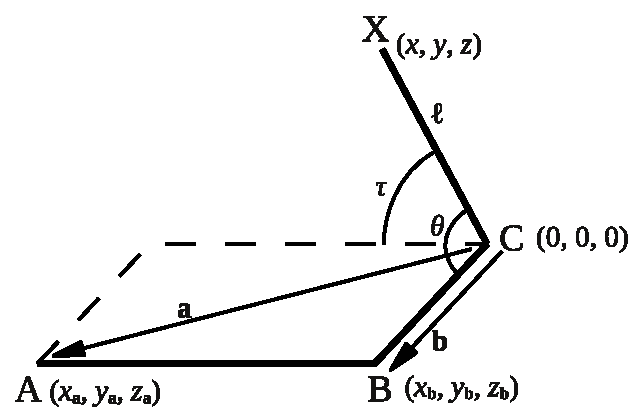
\includegraphics[width=3.5in]{figures/atom_placement}}
\noindent {\small Schematic drawing of the placement of an atom relative to three reference atoms A, B, and C. Atom C is assumed to be at the origin. The vector from C to B is denoted by $\mathbf{b}$, with coordinates $(x_\mathbf{b}, y_\mathbf{b}, z_\mathbf{b})$. Similarly, the vector from C to A is denoted by $\mathbf{a}$, with coordinates $(x_\mathbf{a}, y_\mathbf{a}, z_\mathbf{a})$. The distance from C to X is $\ell$, the angle between CB and CX is $\theta$, and the dihedral angle between ABC and CX is $\tau$.}
\bigskip


\noindent Here, the constants $I$, $J$, and $K$ are coefficients of the target plane, and are obtained from the cross product of vectors $\mathbf{a}$ and $\mathbf{b}$:
\begin{eqnarray} 
I&=&(y_{\bf a}z_{\bf b})-(z_{\bf a}y_{\bf b}), \label{eq:I} \\
J&=&(z_{\bf a}x_{\bf b})-(x_{\bf a}z_{\bf b}), \label{eq:J}\\
K&=&(x_{\bf a}y_{\bf b})-(y_{\bf a}x_{\bf b}). \label{eq:K}
\end{eqnarray}
Solving for $x$, $y$, and $z$ yields the following expressions:
\begin{align}
x&= \frac{R-I J P y_{\bf b}+P K (K x_{\bf b}-I z_{\bf b})+J^2 P x_{\bf b}}{Q}, \label{eq:X}\\
y&= \frac{-I (Rz_{\bf b}+J^2 P x_{\bf b} z_{\bf b}-J P K x_{\bf b} y_{\bf b})+K [R x_{\bf b}-P (J z_{\bf b}-K y_{\bf b})^2]+I^2 P y_{\bf b} (J z_{\bf b}-K y_{\bf b})}{Q(J z_{\bf b}-K y_{\bf b})}, \label{eq:Y}\\
z&= \frac{I R y_{\bf b}-J R x_{\bf b}+I^2 P z_{\bf b} (J z_{\bf b}-K y_{\bf b})+I P K x_{\bf b} (K y_{\bf b}-J z_{\bf b})+J P (J z_{\bf b}-K y_{\bf b})^2}{Q(J z_{\bf b}-K y_{\bf b})}, \label{eq:Z}
\end{align}
where constants $Q$ and $R$ are defined as
\begin{align}
Q&=I^2 (y_{\bf b}^2+z_{\bf b}^2)+J^2 (x_{\bf b}^2+z_{\bf b}^2)+K^2 (x_{\bf b}^2+y_{\bf b}^2)-2 J y_{\bf b} (I x_{\bf b}+K z_{\bf b})-2 I K x_{\bf b} z_{\bf b}, \label{eq:denom}\\
R&=\sqrt{(J z_{\bf b}-K y_{\bf b})^2 [Q\ell^2-P^2 (I^2+J^2+K^2)]}. \label{eq:const}
\end{align}
As we can see from the denominator in Equations \eqref{eq:Y} and \eqref{eq:Z}, the expressions for $y$ and $z$ are undefined if both $y_{\bf b}$ and $z_{\bf b}$ are zero. In this case, the appropriate solution is 
\begin{align}
y&=\frac{ -IJx+S}{J^2+K^2}, \label{eq:Yalt}\\
z&=\frac{ -IK^2x+JS}{K(J^2+K^2)}, \label{eq:Zalt}
\end{align}
with $x$ given by equation~\eqref{eq:X} and $S$ defined as
\begin{equation}
S=\sqrt{K^2[-I^2x^2+J^2K^2(\ell-x)(\ell+x)]}.\label{eq:const2}
\end{equation}
These equations for $x$, $y$, and $z$ yield two possible solutions; the first corresponds to a dihedral angle of $0^\circ$ from $ABC$, and the second corresponds to a dihedral angle of $180^\circ$ from $ABC$. We arbitrarily selected one of these solutions. We then rotated the point X around $\mathbf{b}$ until it was located at the appropriate dihedral angle $\tau$ relative to ABC.

Once atom X is placed at position $(x, y, z)$, we translate these coordinates back to the original coordinate system in which C is not at the origin.


\end{document}

